\documentclass{homework}
\usepackage{homework}
\usepackage{multicol}
\usepackage{cite}

\title{Redes Complexas - CPS765 -%%
	Relatório - 1ª Prática}
\author{Pedro Maciel Xavier}
\register{116023847}
\begin{document}
	
	\smaketitle
	\vspace*{-5pt}
	As redes analisadas foram retiradas do repositório \textit{"Network Science Textbook"}\cite{barabasi:20}, do \textit{Albert-László Barabási}. As quatro redes utilizadas foram: \texttt{protein}, \texttt{metabolic}, ** e **. Para cada grafo foi incluída uma breve descrição, baseada naquela que acompanha os arquivos. Em seguida, consta uma representação gráfica da rede assim como os gráficos das métricas avaliadas: O grau dos vértices, as distâncias entre os pares, o tamanho das componentes conexas e a centralidade (\textit{betweenness}). As estatísticas mais relevantes estão anotadas sobre os gráficos das distribuições empíricas no formato
	$$\text{média} ~ (\text{mediana}) \pm \text{desvio padrão} \in [\text{mínimo}, \text{máximo}]$$
	Além disso, os gráficos das distribuições dos graus dos vértices e dos tamanhos das componentes conexas foram desenhados com o eixo $x$ em escala logarítmica, para melhor visualização. A biblioteca de análise de redes utilizada foi a \texttt{graph-tool}\cite{peixoto:14}, do Tiago Peixoto.
	\vspace*{-5pt}
	\vspace*{-5pt} 	
	\section{Proteínas (\texttt{protein})}	
	\begin{multicols}{2}
	\begin{fig}[\texttt{protein}]
		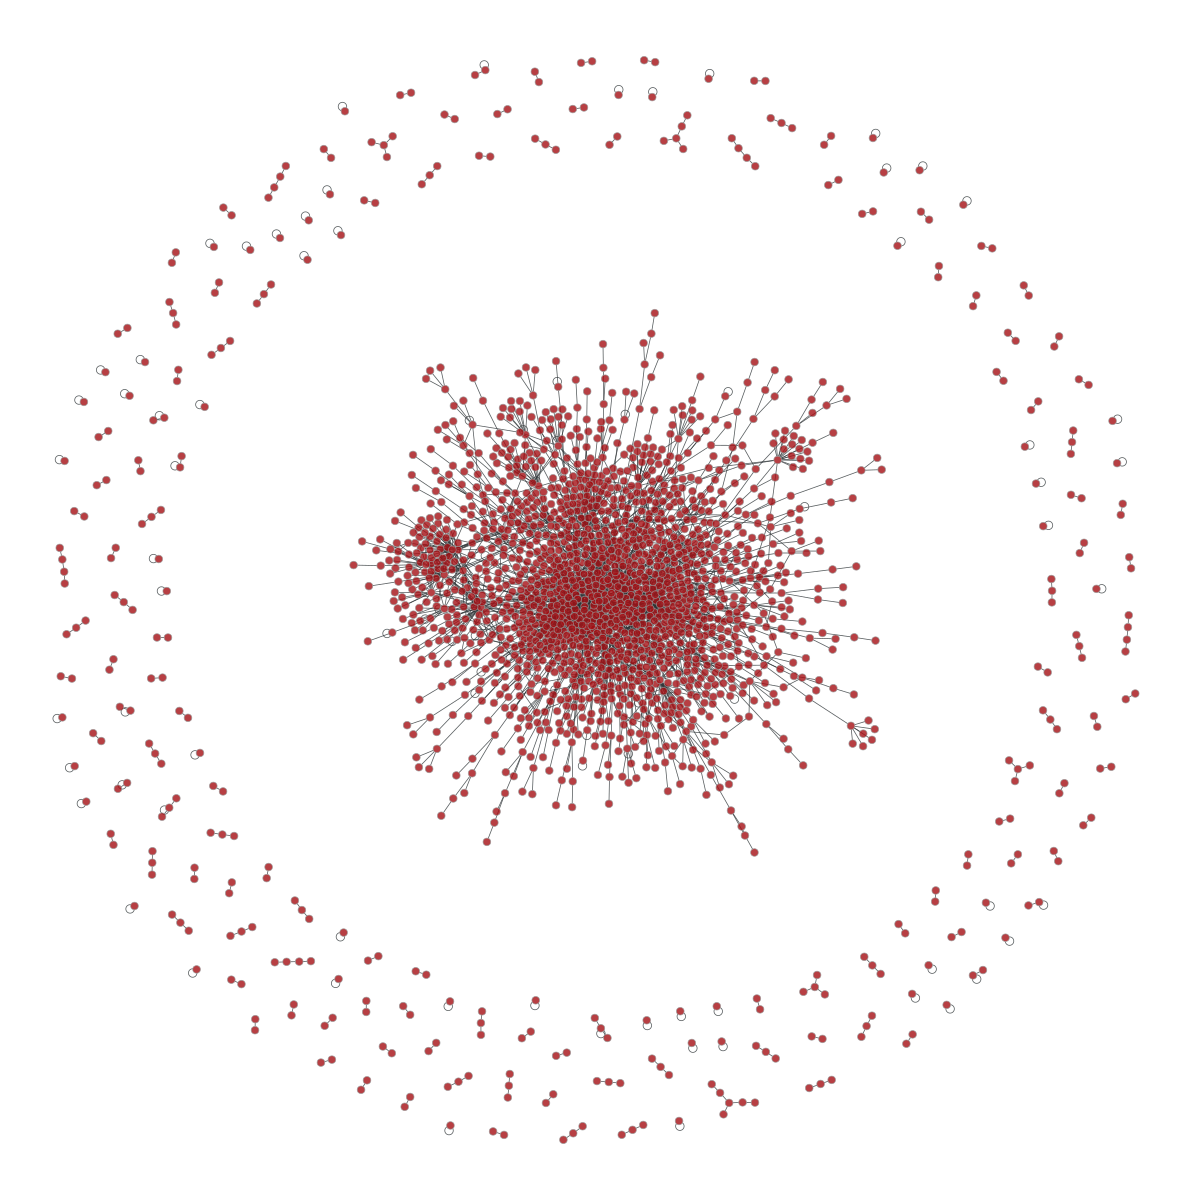
\includegraphics[width=0.15\textwidth]{../results/protein-graph.png}
	\end{fig}

	A rede \texttt{protein} representa as interações entre pares de proteínas em leveduras. Cada vértice corresponde a uma proteína. Cada aresta informa se o par de proteínas interage no interior das células.
	\end{multicols}
	
	\begin{fig}
		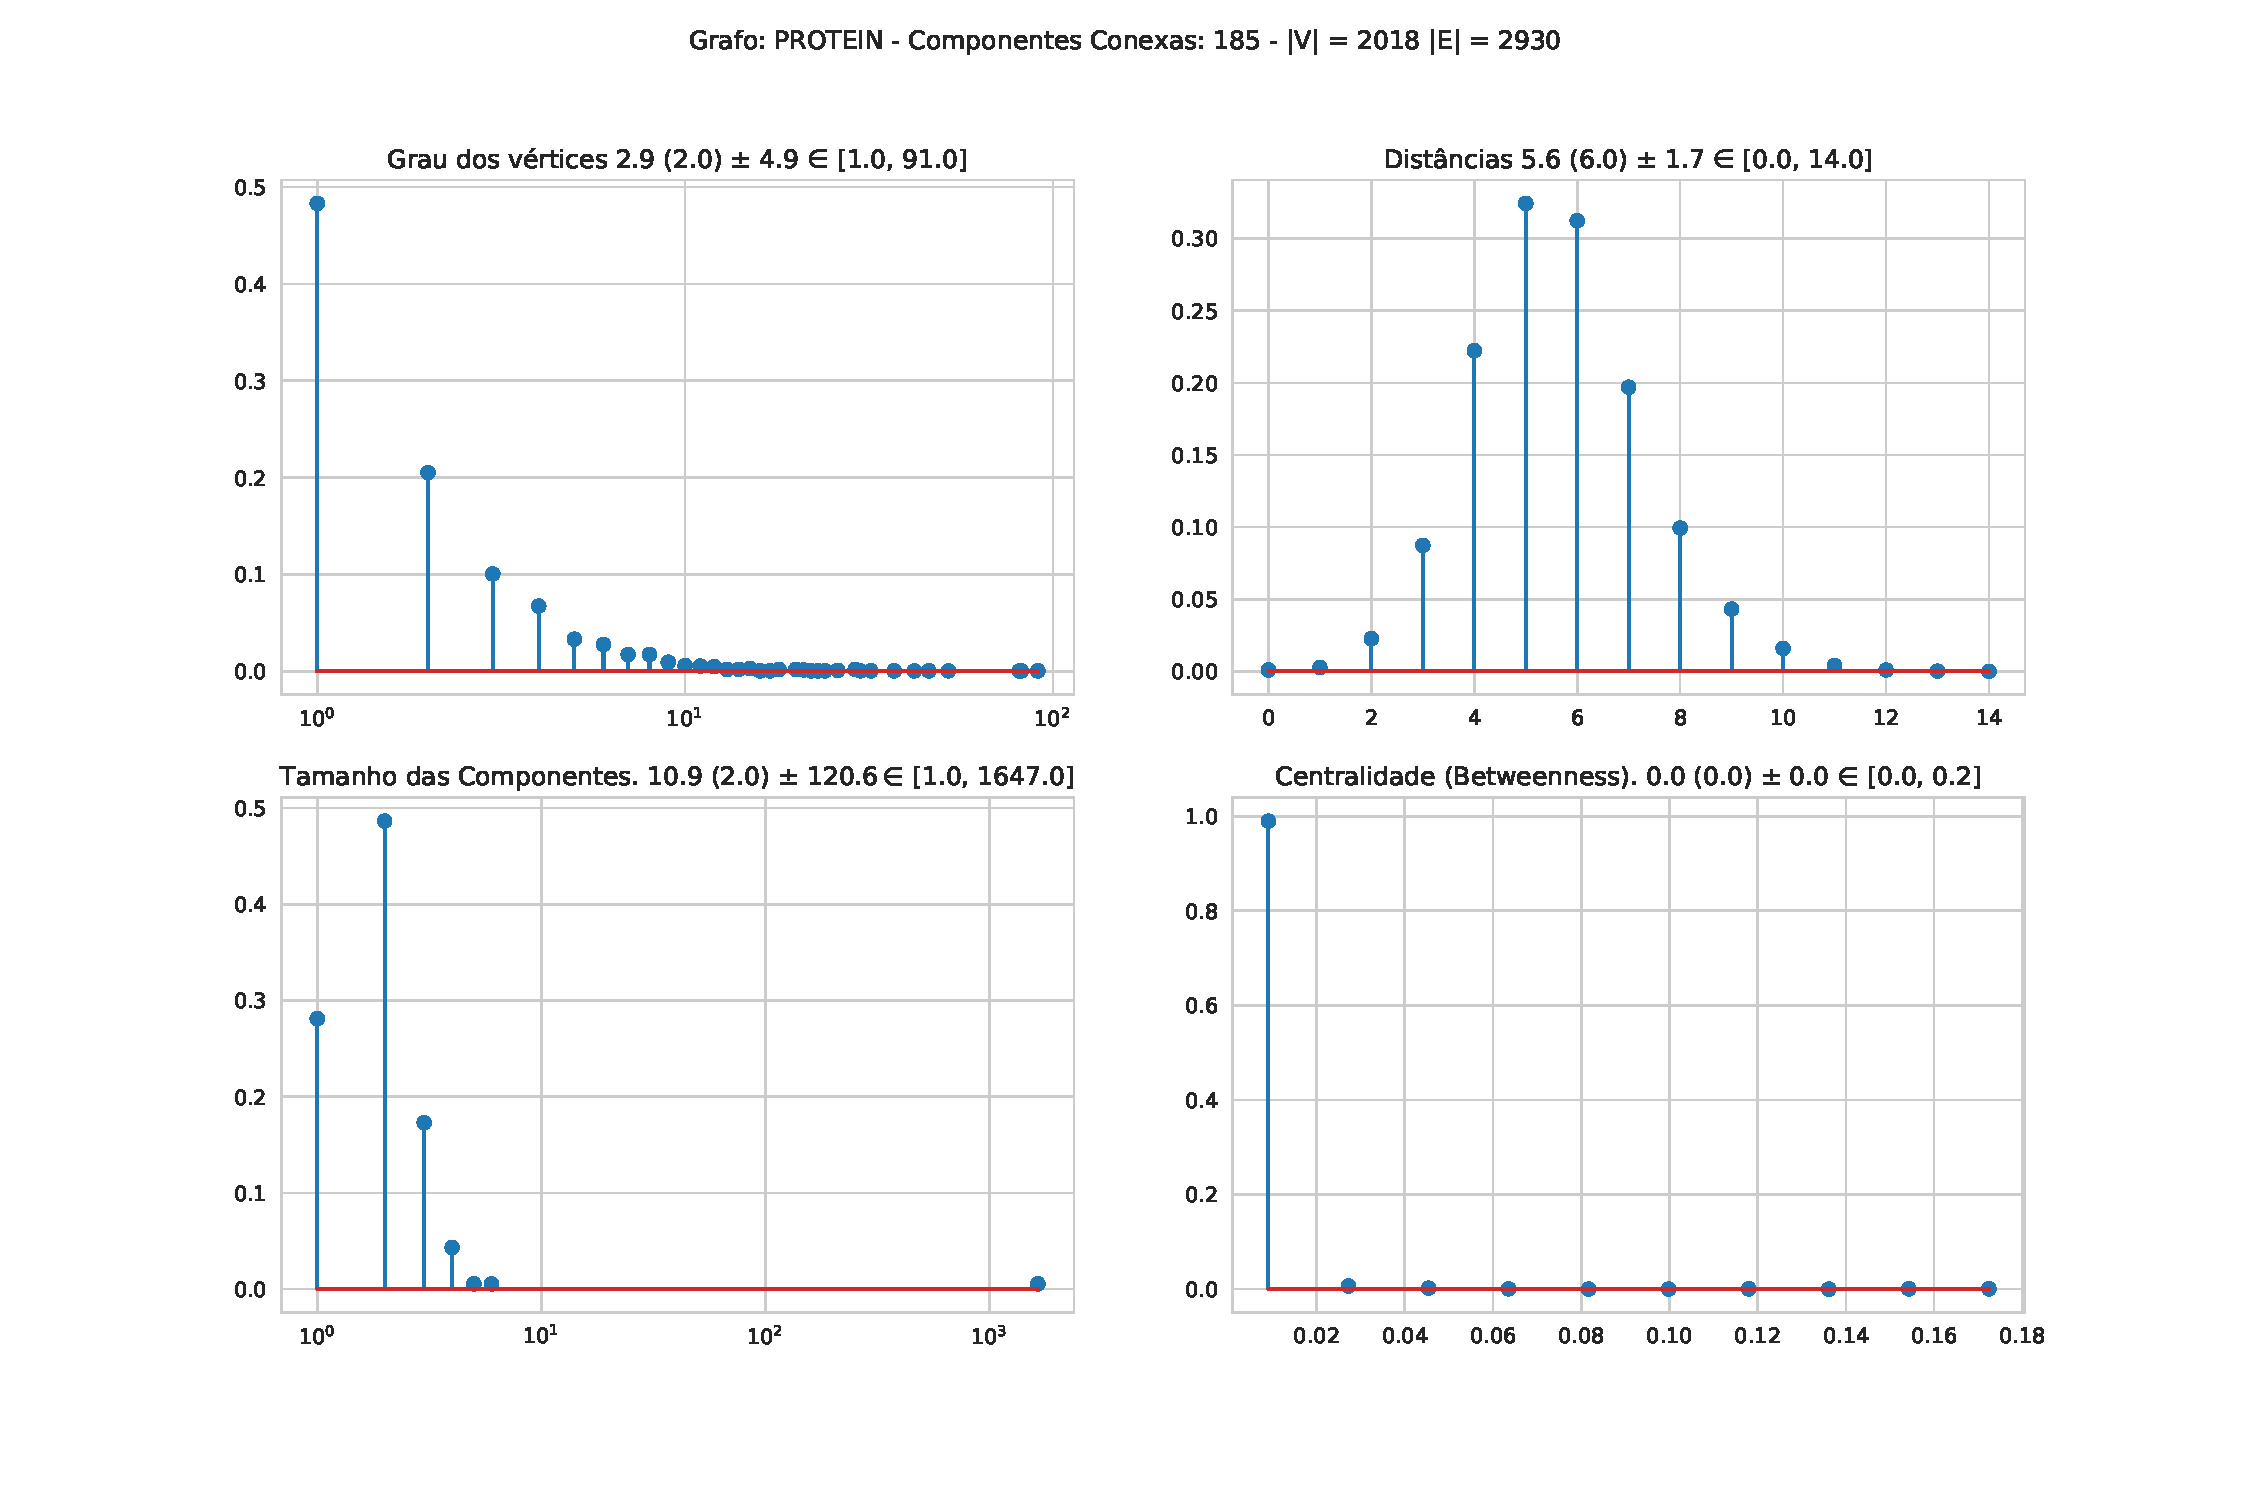
\includegraphics[width=\textwidth]{../results/protein-data.pdf}
	\end{fig}
	
	Esta rede é caracterizada por uma grande componente central com 1637 vértices (cerca de 80\% do total) enquanto o restante das proteínas costuma interagir em pares ou até mesmo não interage com as demais. A centralidade da rede também não é muito alta, assim como a distância média e máxima entre os pares de vértices.
	
		
	\section{Metabolismo \texttt{metabolic}}
	
	\begin{multicols}{2}
		\begin{fig}[\texttt{metabolic}]
			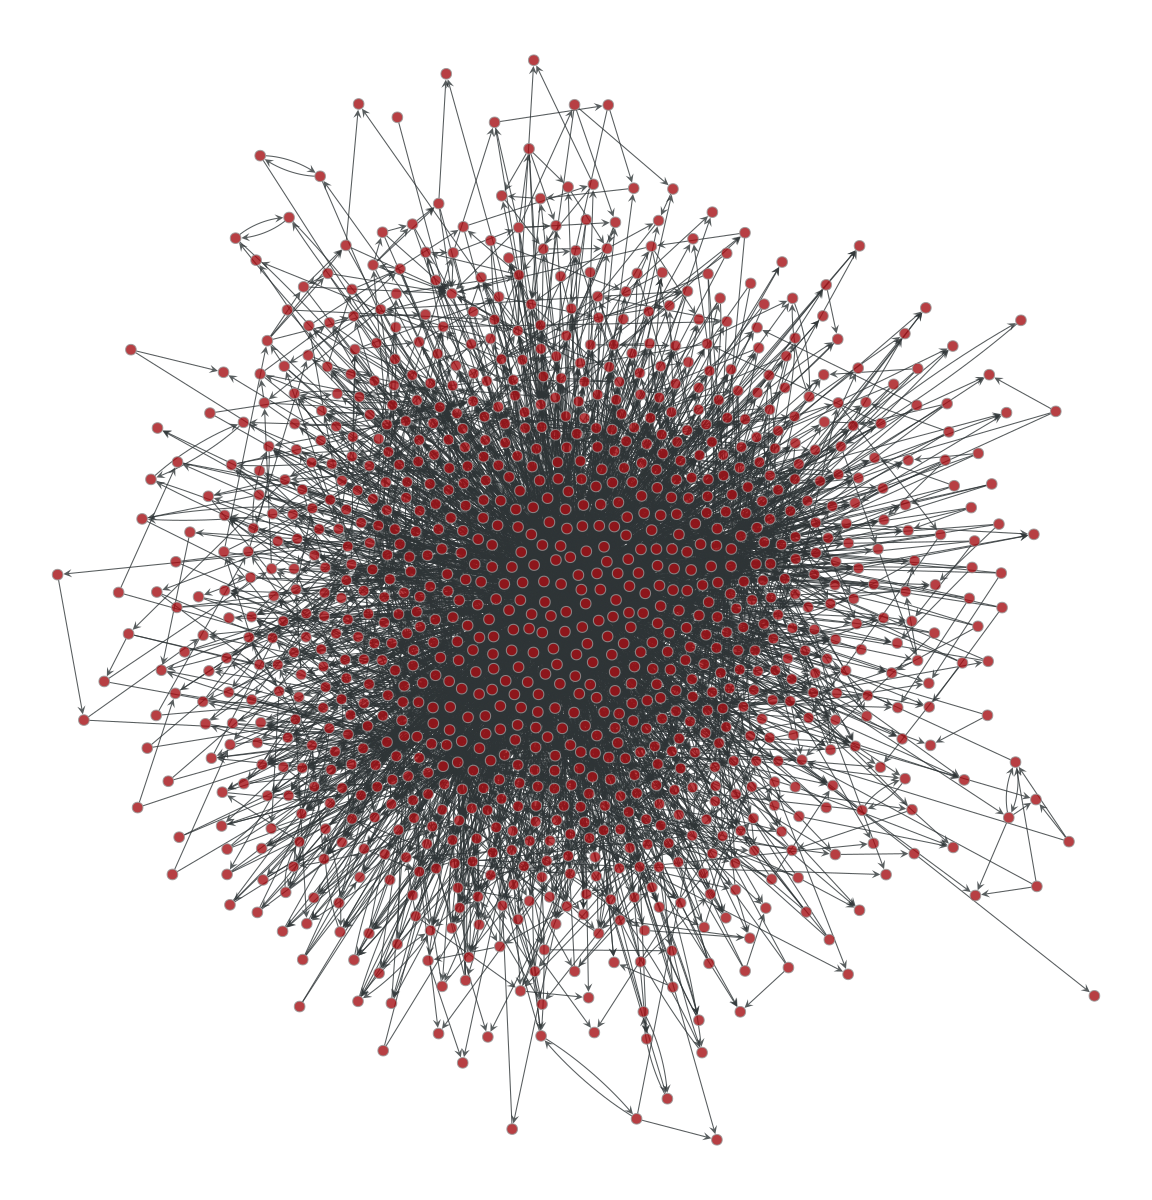
\includegraphics[width=0.2\textwidth]{../results/metabolic-graph.png}
		\end{fig}	
		
		Esta rede descreve as reações metabólicas da bactéria \textit{Escherichia coli}. Cada vértice representa uma substância. O grafo é direcionado de modo que cada aresta diz que há uma reação onde o vértice de saída é um reagente e o de incidência é produto.
	\end{multicols}
	
	\begin{fig}
		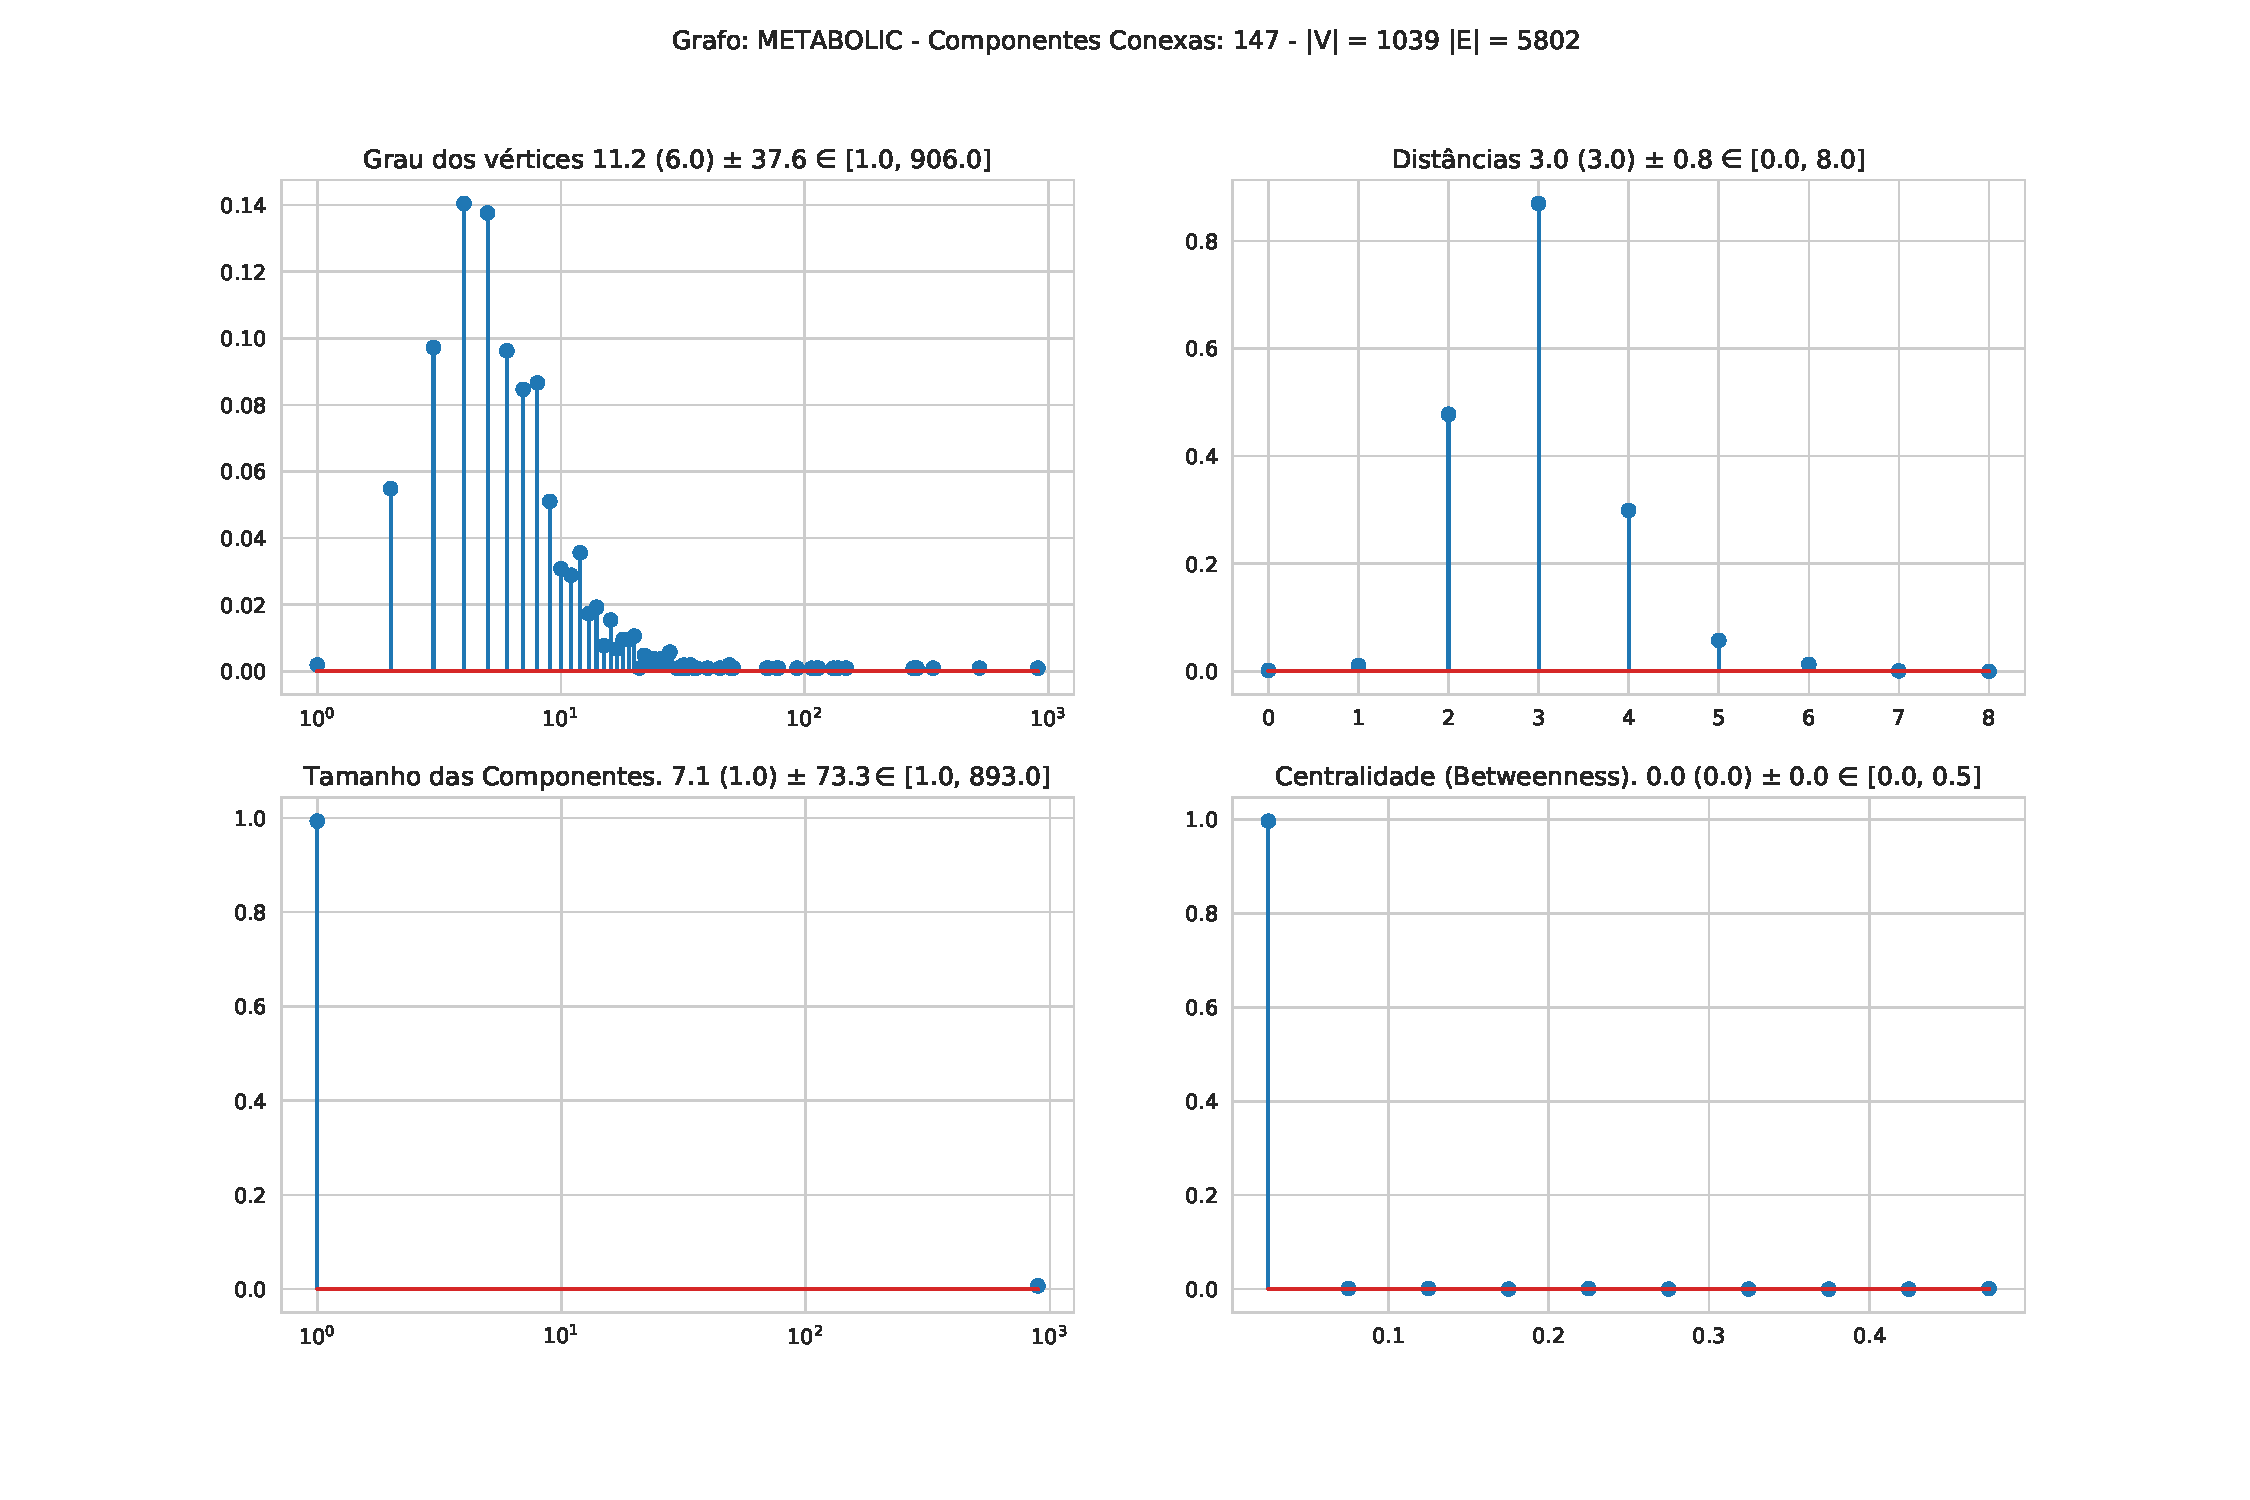
\includegraphics[width=\textwidth]{../results/metabolic-data.pdf}
	\end{fig}

	A observação desta rede direcionada revela que existe uma grande componente conexa central cercada por diversas componentes periféricas. Uma coisa interessante é que algumas proteínas parecem participar em muitos dos processos metabólicos representados, mostrando assim graus muito elevados (em torno de 900). As distâncias, no entanto, não são muito altas, ao contrário da medida de centralidade bastante expressiva (em torno de 0.5).
	
	\section{Rede Elétrica \texttt{powergrid}}
	
	\begin{multicols}{2}
		\begin{fig}[\texttt{powergrid}]
			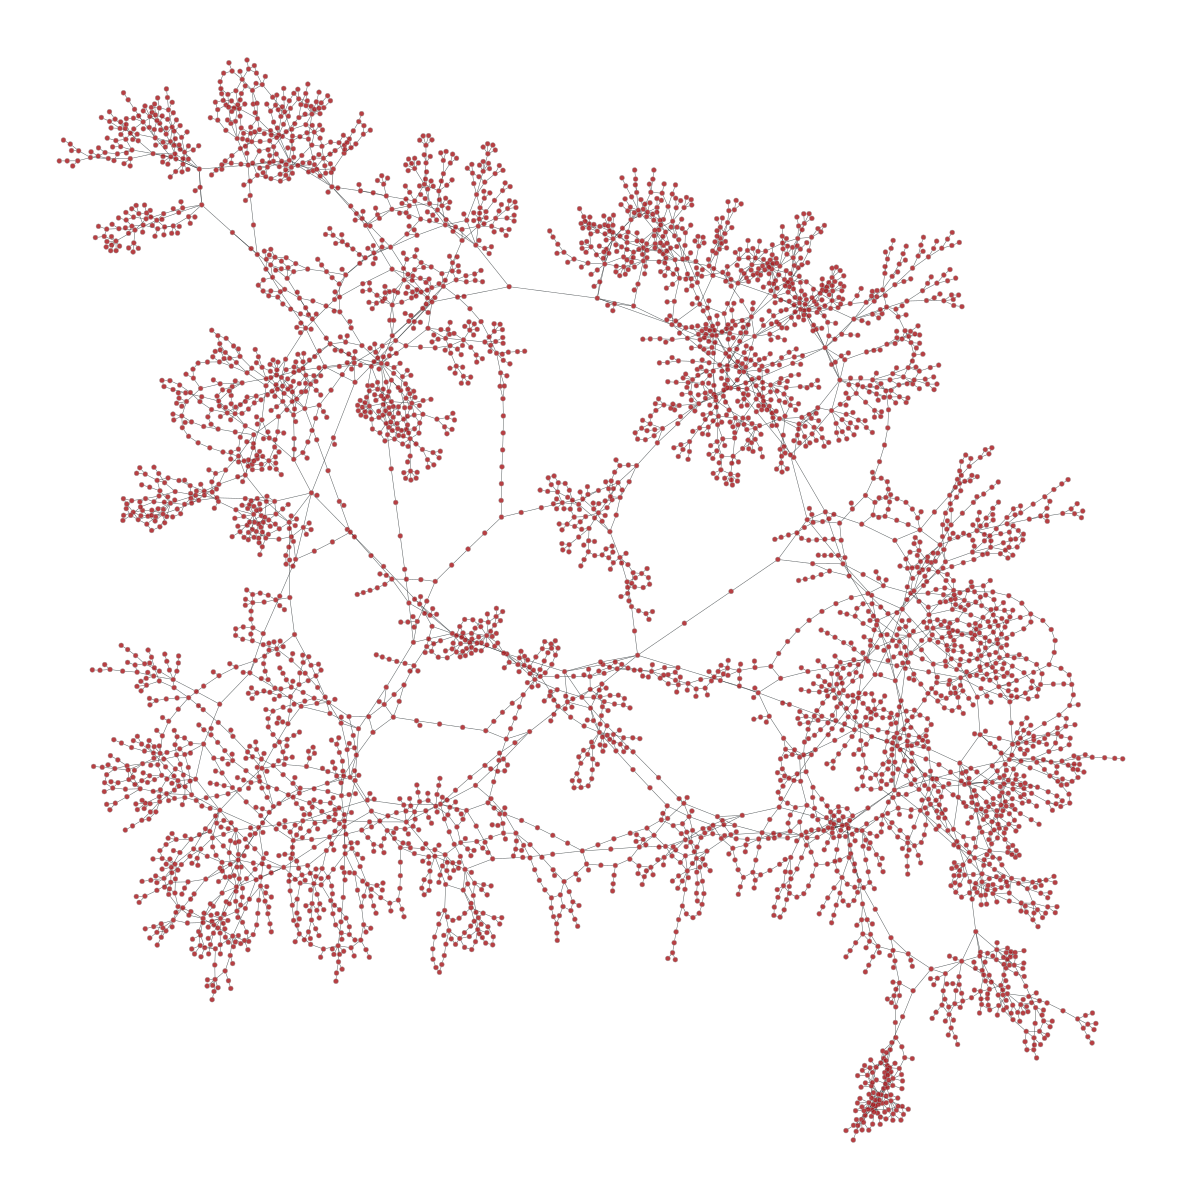
\includegraphics[width=0.15\textwidth]{../results/powergrid-graph.png}
		\end{fig}
		
		Este grafo representa a rede elétrica do oeste dos Estados Unidos. Cada vértice pode ser uma estação, transformador ou consumidor conectado ao serviço de energia. Cada aresta representa um cabo físico ativo.
		
	\end{multicols}
	
	\begin{fig}
		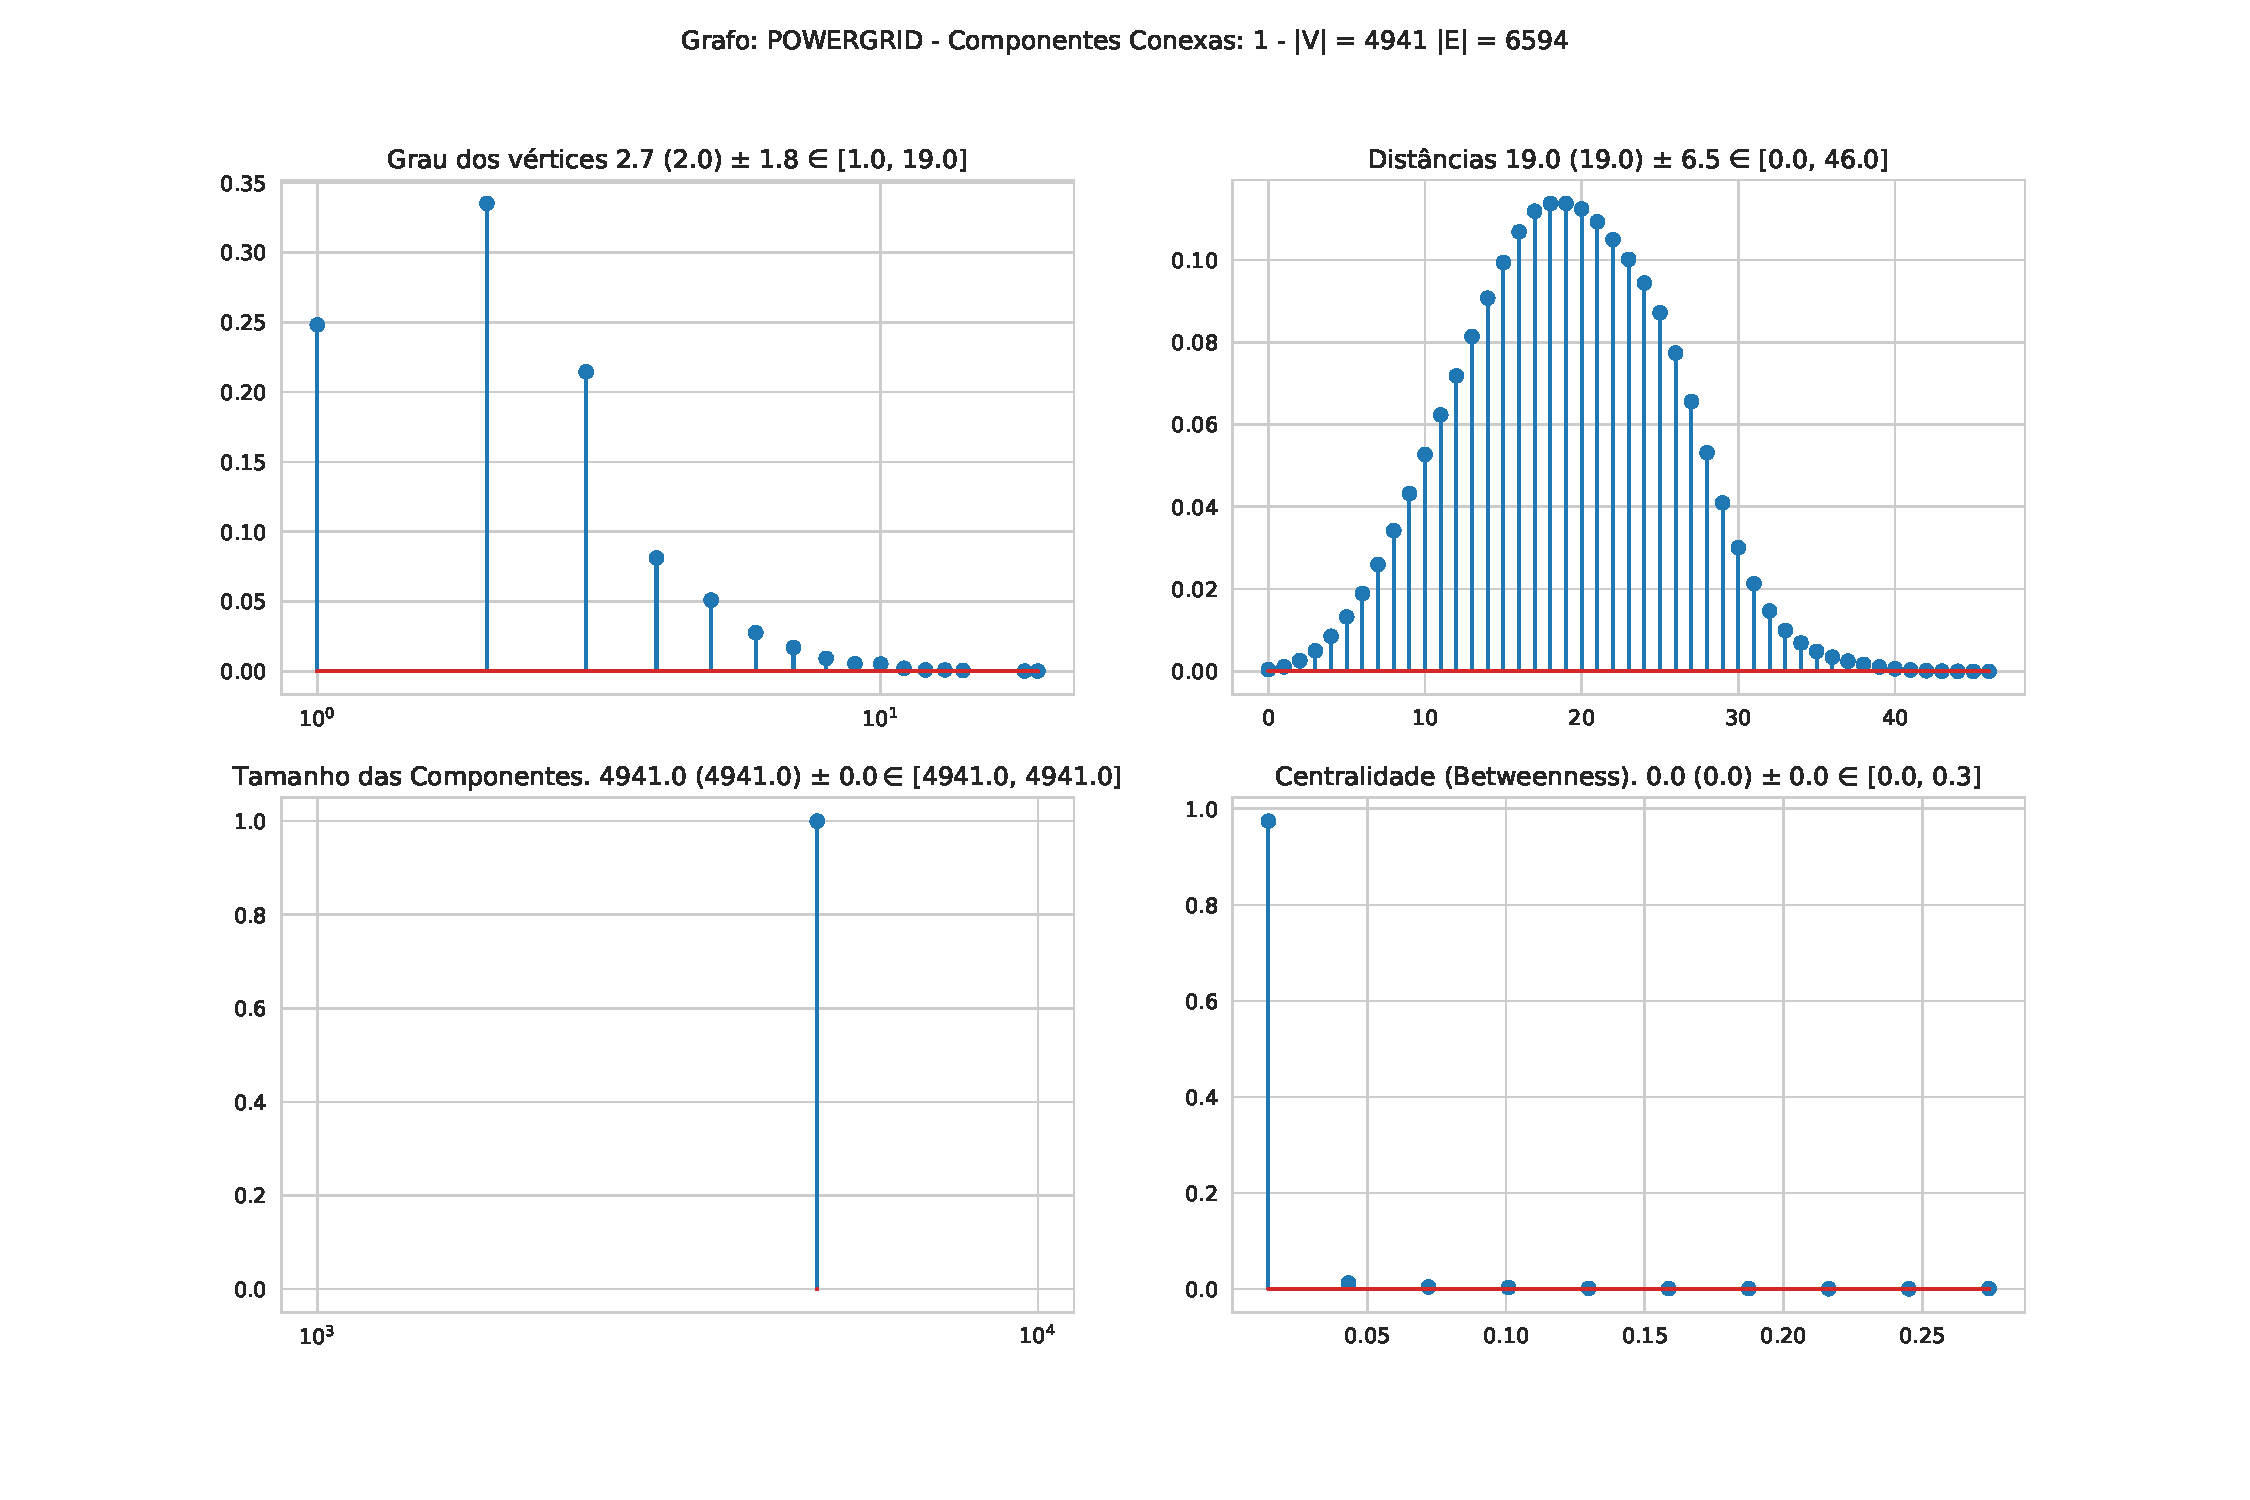
\includegraphics[width=\textwidth]{../results/powergrid-data.pdf}
	\end{fig}
	
	O que as métricas nos revelam é que esta é uma rede formada por uma única componente conexa, ou seja, todos os vértices se encontram conectados por meio de outros. O grau médio reduzido (em torno de 2.7) aliado às altas distâncias (em torno de 19 com máximo em 46) nos leva a crer que o grafo é composto, em grande parte, por subgrafos em forma de árvore. Como era de se esperar pelas malhas energéticas que conhecemos, alguns pontos possuem centralidade mais elevada, o que se verifica na análise.
	
	\section{Colaborações \texttt{collaboration}}
	
	\begin{multicols}{2}
		\begin{fig}[\texttt{collaboration}]
			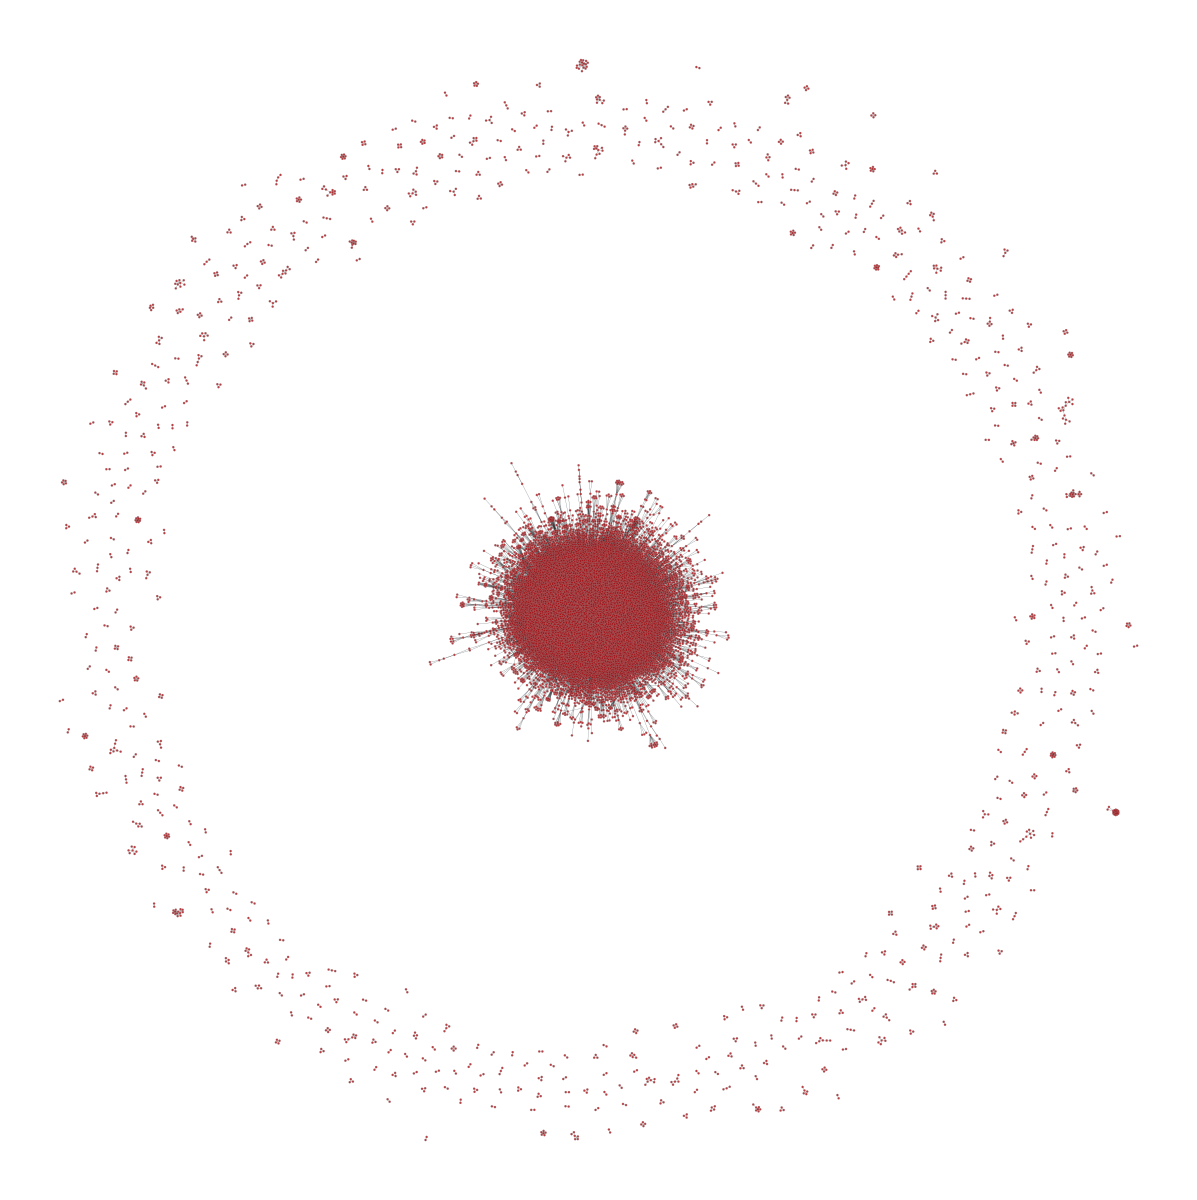
\includegraphics[width=0.2\textwidth]{../results/collaboration-graph.png}
		\end{fig}
	
		Esta rede foi construída com base na colaboração científica entre físicos que estudam a matéria condensada através da plataforma \textit{arXiv} durante 10 anos. Cada vértice representa um autor de algum artigo submetido ao site. Cada aresta indica se dois cientistas foram coautores em algum \textit{paper}.
	\end{multicols}
	
	
	\begin{fig}
		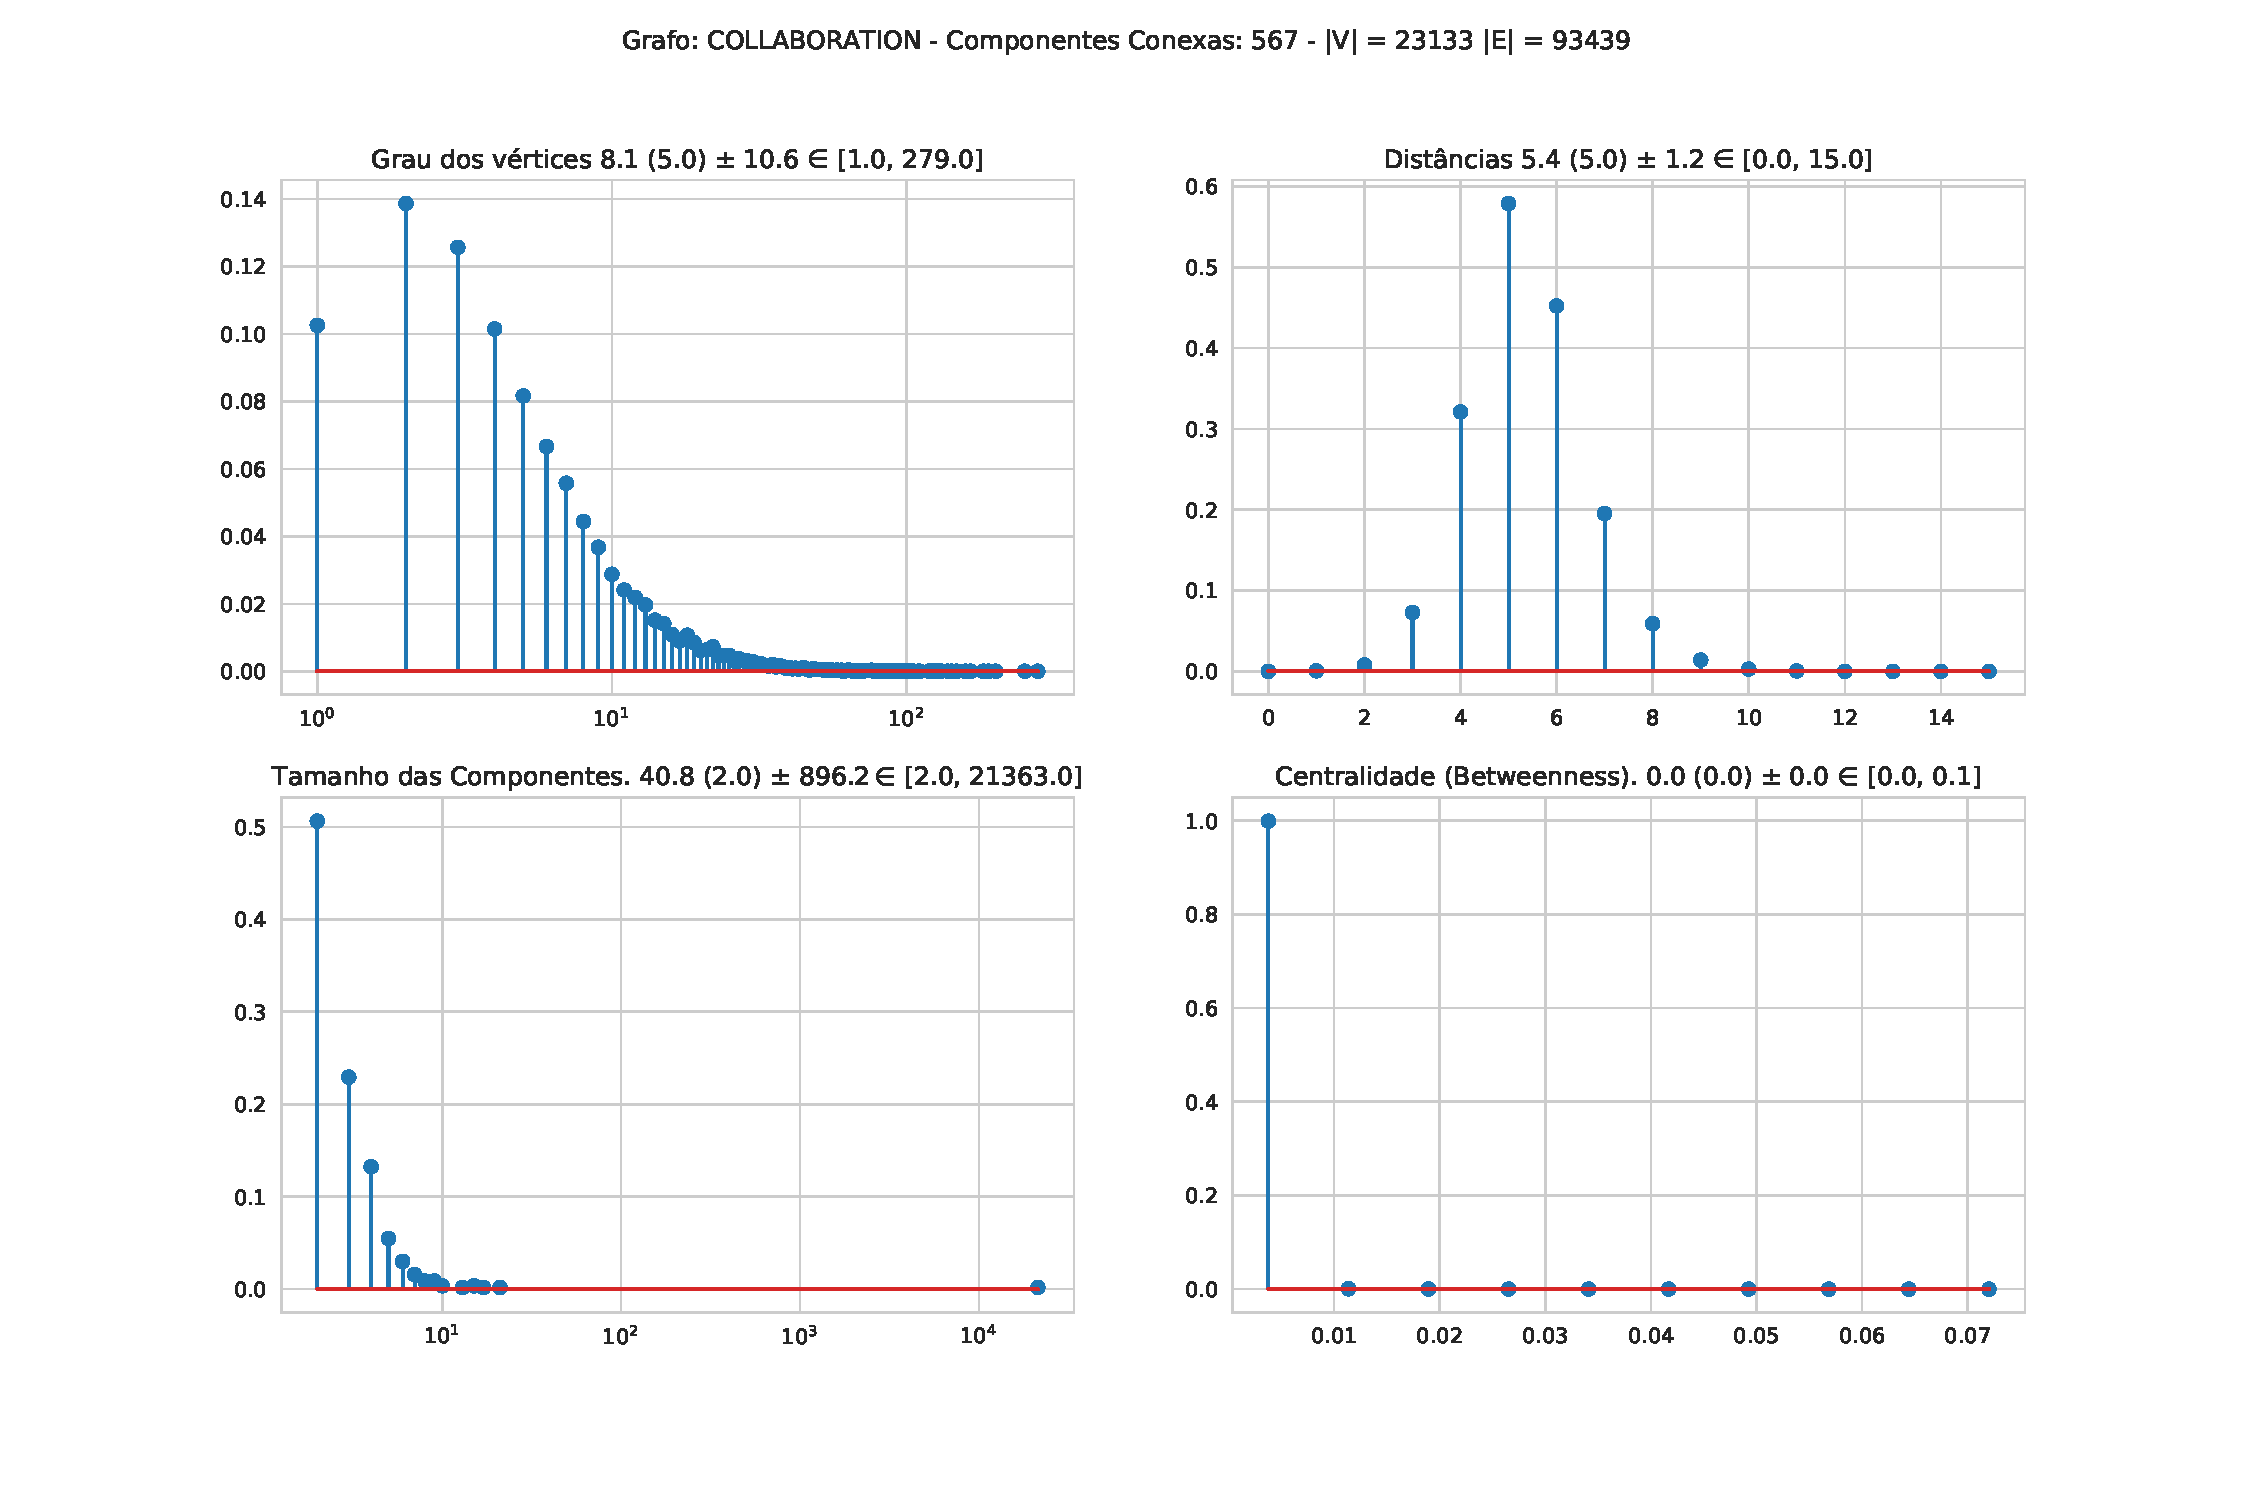
\includegraphics[width=\textwidth]{../results/collaboration-data.pdf}
	\end{fig}

	Na rede de colaborações, vemos uma grande componente central (muito isolada no gráfico dos tamanhos) que abarca a gigantesca maioria dos pesquisadores. Além disso, temos outras componentes conexas periféricas, que não chegam as centenas de cientistas em cada. Aqui se verifica um cenário de \textit{mundo pequeno} onde a distância média entre dois pesquisadores é de apenas 5.4, podendo chegar a, no máximo, 15. A centralidade dos vértices também não é muito elevada. É interessante como estas características da rede se parecem com a das proteínas nas leveduras.

	\bibliography{practice1}{}
	\bibliographystyle{plain}

\end{document}